\newpage
\chapter{Фотоэффект}
\par Герц в 1887 году провел такой эксперимент: взял запаенный сосуд, 2 электрода, вольтметр и амперметр. Оказалось, что при подаче напряжения наиболее эффективно ток потечет, если 1 из электродов будет находиться под действием  ЭМ-излучения (UV). Источник обсуждать не будем. Причем ток зависит от характеристик этого излучения. На электродах есть заряженные частицы, условно будем называть их электронами. Предположим, что при поглощении падающего света (кака раз ЭМ-волна, которая содержит \textit{E}) происходит раскачка заряженных частиц (движутся в этом поле), тогда они преобретают энергию. Посчитать её - задача сложная, ведь электроны привязаны к атомам, движутся вокруг них, рядом есть еще атомы.

\begin{figure}[h]
\begin{center}
\begin{minipage}[h]{0.3\linewidth}
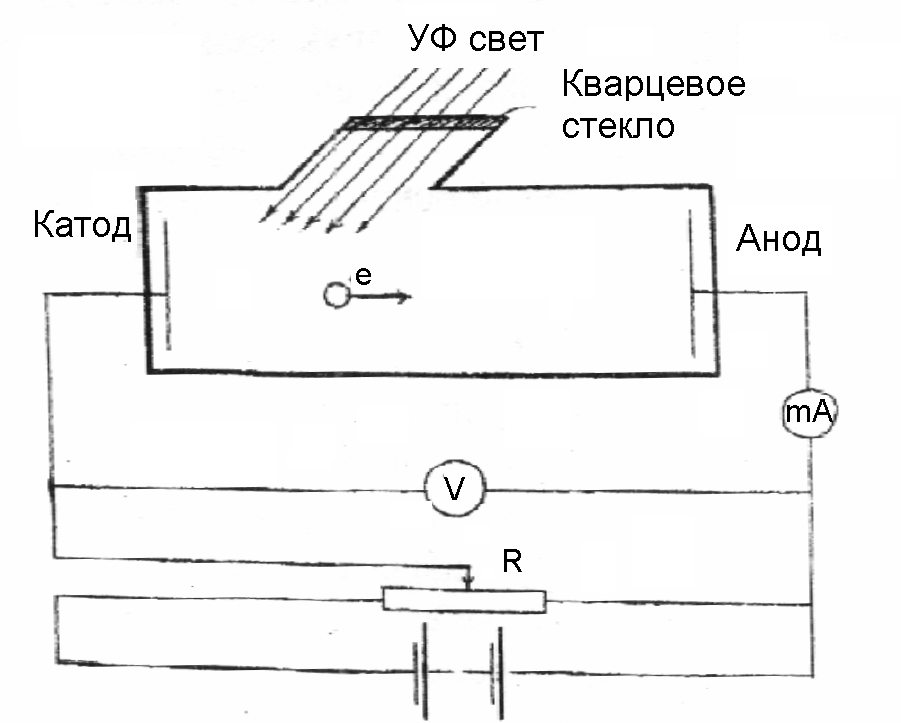
\includegraphics[width=1\linewidth]{pictures/2.png}
\caption{Схема эксперимента} %% подпись к рисунку
\end{minipage}
\hfill
\begin{minipage}[h]{0.3\linewidth}
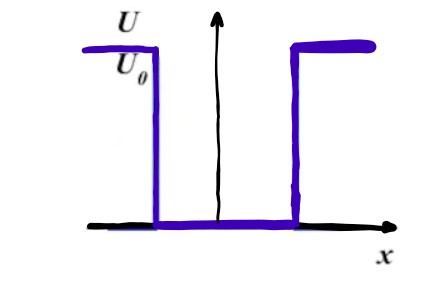
\includegraphics[width=1\linewidth]{pictures/2.1.jpg}
\caption{Потенциальный барьер}
\end{minipage}
\hfill
\begin{minipage}[h]{0.3\linewidth}
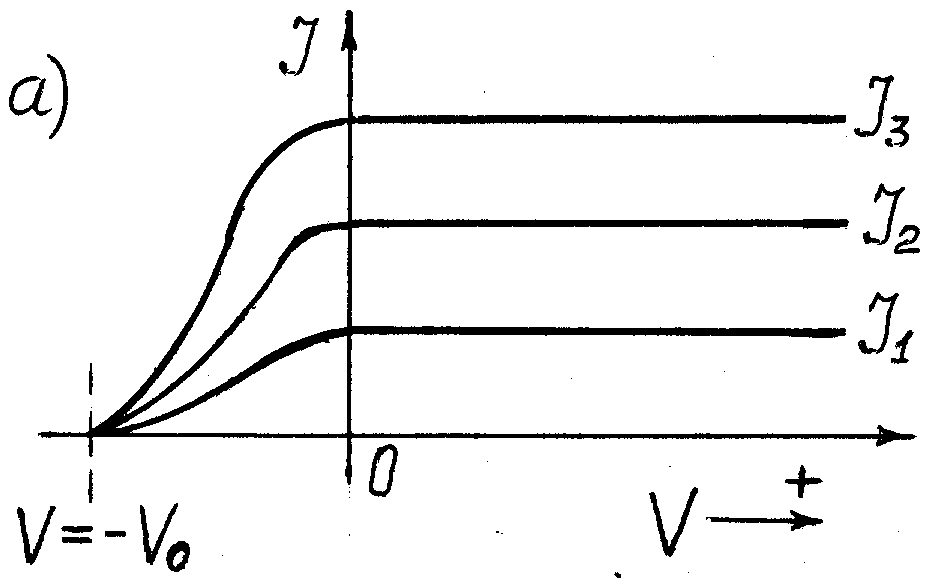
\includegraphics[width=1\linewidth]{pictures/2.2.png}
\caption{Зависимость фототока от напряжения}
\end{minipage}
\end{center}
\end{figure}


Но с точки зрения потенциала \textit{U} электрод - это ящик. Вообще есть и потенциалы атомов, действующих на этот электрод, забудем про них. Что бы вылететь, электронам необходимо преодолеть этот потенциальный барьер.
\par Пусть  $E \sim e^{i w t}$, тогда уравнение Ньютона будет выглядеть следующим образом (не забываем, что это грубая прикидка)
 $m a =e E_0 e^{i w t}$. Уравнение линейное, работать удобнее с комплексными экспонентами, в итоговом выражении возьмем действительную часть. Отсюда можем определить, что $v \sim e^{i w t}$, а ее амлитуда:
$$v_0 \simeq \frac{e E_0}{w m} \shortrightarrow E_{кин} = \frac{m e^2 E_0^2}{2m^2 w^2}=\frac{e^2 E_0}{2 m w^2} $$

\par Т.е. при низкой $w$ электроны быстро улетят, а поскольку приложено напряжение, потечет ток, но при облучении радиочастотной волной (от 3 кГц до 3000 ГГц) ничего не произойдет. На самом деле люди измеряют фототок как линейную функцию интенсивности $P=E_0^2$. С другой стороны, если измерить фототок в зависимости от поданного напряжения, то график окажется другим. Рассмотрим Рис.2.3, где три кривые обозначают три разные значения интенсивности: ток течет в случае $ I(V=0) \ne  0 $ (светим на определенный электрод, видимо, электроны там так выбились, что некоторые из них "на издыхании" долетели до 2 электрода, дали немножко тока), далее, прикладываем напряжение отрицательное, т.е. которое мешает движению частиц, лампа запирается, ток обращается в ноль. Запирающее напряжение не зависит от интенсивности облучения \textit{P}, что странно. Увеличивая  \textit{P}, мы увеличиваем количество выбитых электронов, рассмотрим $|U_0|$ как функцию частоты: она растет с некоторого порогового значения $w_п$- границы всего эффекта.

 \begin{wrapfigure}[12]{r}{0.4\linewidth} 
\vspace{-2ex}
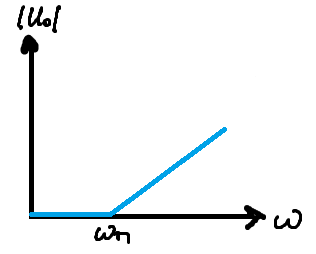
\includegraphics[width=0.7\linewidth]{pictures/2.3.png}
\caption{$|U_0|(w)$}
\end{wrapfigure}

 \par Запирающее напряжение в некотором смысле - мера энергии, которую мы сообщаем электрону при облучении, чтобы он вылетел, часть энергии может быть и остается, чтоб он куда-то летел. Эту самую избыточную энергию начинаем "душить", создавая противодействующую его движению туда. Запирание в этом смысле - явление, когда электрон мог преодолеть потенциальный барьер, но никуда не полетел, ток не пошел. Значит, существует какая-то красная граница фотоэффекта (т.к. для низких частот, а красный свет ниже всех по частоте). Вообще не понятно, почему это зависит от частоты, тем более таким образом.

\par Если свет может излучаться/поглощаться порциями (квантами) с энергией $E= \hbar w$, то ситуация получается простая: энергия, которую имеет квант света, тратится на некоторую величину, называемой работой выхода (это та самая величина потенциальной энергии, необходимая для преодоления барьера), вместе с остаточной кинетической энергией они связаны соотношением $\hbar w = A_e + E_k$. Энергия отсечки (когда кинетическая энергия обращается в ноль и ее не хватает для преодоления вышеупомянутого барьера) здесь такая, что $\hbar w \leq A_e $.
